\documentclass[12pt,a4paper]{article}

\usepackage[utf8]{inputenc}
\usepackage[T2A]{fontenc}
\usepackage{cyrtimes}
\usepackage[russian]{babel}
\usepackage{amsmath}
\usepackage{amsfonts}
\usepackage{amssymb}
\usepackage{graphicx}
\usepackage[left=3cm,right=1.5cm,top=2cm,bottom=2cm]{geometry}
\usepackage[titletoc]{appendix}
\usepackage{multicol}
\usepackage[labelsep=endash]{caption}

\author{Тумашик Игорь Александрович}
\title{Полутоновые матричные штрихкоды}

\pdfcompresslevel=9

\begin{document}

\renewcommand{\figurename}{Рисунок}
\renewcommand{\appendixname}{ПРИЛОЖЕНИЕ}

%titlepage
\titlepage
\begin{center}
	\begin{large}
		\textbf{МИНИСТЕРСТВО~ОБРАЗОВАНИЯ~РЕСПУБЛИКИ~БЕЛАРУСЬ}
		
		\smallskip
		\textbf{БЕЛОРУССКИЙ~ГОСУДАРСТВЕННЫЙ~УНИВЕРСИТЕТ}
		
		\smallskip
		\textbf{Факультет~прикладной~математики и информатики}
		
		\smallskip
		Кафедра~информационных~систем~управления
	\end{large}
\end{center}

\vfill

\begin{center}
	\large {ТУМАШИК ИГОРЬ АЛЕКСАНДРОВИЧ}
	
	\bigskip	
	{\Large \textbf{ПОЛУТОНОВЫЕ МАТРИЧНЫЕ ШТРИХКОДЫ}}
	
	\bigskip
	Дипломная работа
	
	студента 5 курса 2 группы
\end{center}


\vfill
\begin{flushright}
	\begin{minipage}{7cm}
		\textbf{Руководитель:}
		
		\textit{Абламейко Сергей Владимирович}
		
		академик, профессор кафедры ИСУ,
		
		доктор технических наук 
	\end{minipage}
\end{flushright}

\vfill

\begin{center}
	МИНСК
	
	БГУ
	
	2013
\end{center}

\newpage

%abstract
\newcommand{\pagescount}{10}
\section*{АННОТАЦИЯ}

\textit{Тумашик И. А}. Полутоновые матричные штрихкоды:
Дипломная работа~/ Минск: БГУ, \\ 2013.~--- \pagescount~с.

\medskip


\section*{АНАТАЦЫЯ}

\textit{Tумашык І. А.} Паўтонавыя матрычныя штрыхкоды:
Дыпломная работа~/ Мінск: БДУ, \\ 2013.~--- \pagescount~c.

\medskip


\section*{ANNOTATION}

\textit{Tumashyk I. A.} Grayscale matrix barcodes:
Dyploma~/ Minsk: BSU, 2013~--- \pagescount~p.

\medskip

\newpage

%summary
\section*{РЕФЕРАТ}

Дипломная работа, \pagescount\ с., ? рис., 
%** табл.,
? источников. 

\medskip
\textbf{Ключевые слова:} ШТРИХКОД, МАТРИЧНЫЙ ШТРИХКОД, 
РАСПОЗНАВАНИЕ ОБРАЗОВ, ОБРАБОТКА ИЗОБРАЖЕНИЙ.

\medskip
\textbf{Объект исследования} --- матричные штрихкоды, полутоновые штрихкоды.

\textbf{Цель работы} --- разработать спецификацию полутонового матричного 
штрихкода, предложить реализацию.

\textbf{Методы исследования} --- методы прикладной математики и информатики, 
технология программирования.

\textbf{Результат исследования} --- разработан полутоновый матричный 
штрихкод, представлена реализация. 

\textbf{Областью применения} являются системы использующие автоматическую
идентификацию объектов находящихся в прямой видимости.

\newpage

%contents
\renewcommand{\contentsname}{СОДЕРЖАНИЕ}
\tableofcontents

\newpage
\listoffigures
\listoftables
\newpage



%introduction
\section*{ВВЕДЕНИЕ}
\addcontentsline{toc}{section}{ВВЕДЕНИЕ}

Уже давно вычислительная техника используется не только в прямом 
взаимодействии с другими цифровыми устройствами, но и с предметами,
имеющими аналоговую природу. В частности, в этой работе пойдёт речь о
применении ЭВМ для считывания графических данных, 
непосредственно предназначенных 
для этого, посредством устройств ввода изображений. Важным аспектом
является как раз то, что рассматриваемые объекты специально спроектированы
для распознавания их цифровыми устройствами. Среди них особое место 
занимают \textit{штрихкоды}\footnote{В настоящее время очень часто
это слово пишут через девиз (см., например, <<Википедию>>). Однако,
<<Русский орфографический словарь: около 180 000 слов>> под редакцией
Лопатина В.~В. \cite{bib:russkijLopatin} настаивает на слитном написании~--- 
\textit{штрихкод}, в таком виде это слово и будет использовано в работе.}. 

Одной из важнейших характеристик любого штрихкода является площадь
занимаемая на рабочей поверхности. В то же время понятно, что невозможно
бесконечно уменьшать размеры элементов кода (по условиям печати и 
качества распознавания). Вывод напрашивается сам собой: следует
увеличить информативность наименьшего элемента кода, чтобы добиться
уменьшения размера всего штрихкода. Логично использовать для этого
градации яркости~--- от чёрного до белого (тон, всё-таки, очень зависит
от освещённости). Будем такие коды называть \textit{полутоновыми}. 
Ещё более реальной делают эту идею всё возрастающее
мощности цифровых камер различных устройств. Вокруг этой простой 
задумки и построена данная работа. Кроме приведения спецификации 
полутонового кода, рассматриваются существующие разработки в этой 
области, проводиться сравнение с существующими подходами (автору не 
известны другие штрихкоды построенные на этой идеи), приводиться
реализация полутонового штрихкода. 


\section{ОБЗОР СУЩЕСТВУЮЩИХ СТАНДАРТОВ \\ ШТРИХКОДОВ}

\textbf{Штрихкод} (сокр. от <<\textit{штриховой код}>>, англ. 
<<\textit{bar code}>>) --- графическая информация наносимая на 
поверхности предметов, предназначенная для обработки техническими
средствами.

Выделяют две большие группы штрихкодов: \textit{линейные} 
и \textit{двухмерные}.
В первом случае информационную нагрузку имеют только чередования 
участков различной яркости по одной из осей, во втором --- по обеим.


\subsection{\textsc{Линейный штрихкоды}}  

Исторически, линейные штрихкоды появились первыми (50--70-ые годы 
XX века). Коды этой группы не отличаются особым разнообразием ---
чередование чёрных и белых полос, кодирующие цифры либо буквы. Вместе
с тем, линейные коды наносятся практически на все товары 
(\figurename\ \ref{fig:ean}), 
распространяемые в розницу (формат EAN --- European Article Number),
и потому наиболее широко распространены. Другие примеры рисунки 
\ref{fig:code128}, \ref{fig:itf14}. 

В этой работе мы не будем рассматривать линейные штрихкоды.

\begin{figure}[h]
    \begin{multicols}{2}
 
        \begin{center}
             
\includegraphics[scale=0.5]{img/ean_sample} 
             \caption{Штрихкод в формате EAN}
             \label{fig:ean}
        \end{center}
   
        \begin{center}
            
\includegraphics[scale=0.5]{img/ean_sample} 
            \caption{Штрихкод в формате Code 128}
            \label{fig:code128}
        \end{center}       
       
    \end{multicols}
\end{figure}

\begin{figure}[h]
    \centering
    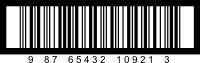
\includegraphics[scale=0.7]{img/itf_sample}
    \caption{Штрихкод в формате ITF-14}
    \label{fig:itf14}
\end{figure}
    
\subsection{\textsc{Двумерные штрихкоды}}

Как уже отмечалось, в двумерных штрихкодах информация кодируется
по обеим осям. Выделяются два вида двумерных кодов: \textit{стековые}
и \textit{матричные}.

\subsubsection{Стековые штрихкоды}  
Стековые штрикоды являются, в некоторой мере, переходным вариантом
между линейными и двухмерными. Они представляю собой строки расположенные
одна под одной. Каждая строка есть ни что иное, как одномерный штрихкод.

Несмотря на свою простоту, данный тип штрихкодов позволяет хранить 
значительные объёмы данных. Например, штрикод формата PDF417 
(см. \figurename\ \ref{fig:pdf417}) может содержать до 2710 знаков.
Стековые штрихкоды также не является объектом рассмотрения данной
работы. 

\begin{figure}[htb]
    \centering
    
\includegraphics{img/pdf417_sample}
    \caption{Штрихкод в формате PDF417}
    \label{fig:pdf417}
\end{figure}

\subsubsection{QR-код}
Ниже будет приведено краткое описание QR-кода. Полное описание можно найти в
спецификации ISO/IEC 18004:2006 \cite{bib:isoQR}.  

QR-код представляет собой квадратную матрицу размером от $21 \times 21$ до 
$170 \times 170$ барселей. Технически выделяют от 1 ($21 \times 21$) до
40 ($170 \times 170$) версии кода (т.е. шаг равен 4).

Каждый барсель есть некоторый 
аналог бита при представлении информации в электронном виде. Среди этих
барселей можно выделить следующие (\figurename\ \ref{fig:qrSimple}): 
\textit{информационные}~--- содержат 
непосредственно данные, \textit{корректирующие}~--- для исправления ошибок
(используются коды Рида-Соломона (см. \ref{sec:RSCode})), 
\textit{заполняющие}~---
дополняют до правильно квадрата, \textit{поисковые шаблоны}~--- 
служат для локации кода при распознавании (хорошо заметные квадраты по 
углам кода, а также чередующие чёрные и белые барсели чуть ниже них), 
\textit{форматные}~--- содержат информацию о структуре кода (в QR-коде 
расположены по периметру поисковых шаблонов). Дополнительно смотрите 
\figurename\ \ref{fig:qrDecode}

\begin{figure}[h]
    \centering
    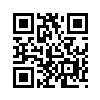
\includegraphics{img/qr_sample}
    \caption{Штрихкод в формате QR-код}
    \label{fig:qrSimple}
\end{figure}

В одном коде можно сохранить до 7084 цифр, либо до 4296 цифр и символов,
либо до 2953 байт произвольных данных, либо до 1817 иероглифов Канджи.

Дополнительно фиксируется уровень коррекции ошибок \textit{L}, 
\textit{M}, \textit{Q}, \textit{H}, что
позволяет восстановить до 7\%, 15\%, 25\%, 30\% данных соответственно.
Рекомендуется использовать уровень \textit{M}.

При распечатке требуется обеспечить белые поля толщиной не менее четырёх
барселей.

\begin{figure}[htb]
    \centering
    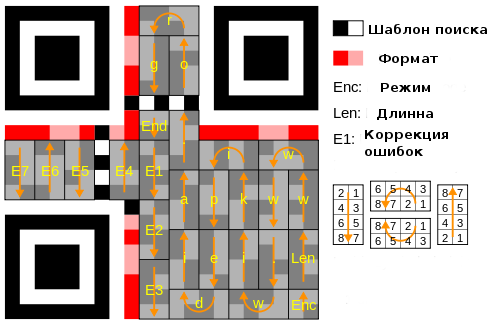
\includegraphics[scale=0.5]{img/qr_decode}
    \caption{Пример декодирования QR-кода}
    \label{fig:qrDecode}
\end{figure}


\subsubsection{Data Matrix}
Data Matrix --- двумерный штрихкод (описывается стандартом 
ГОСТ Р ИСО/МЭК 16022--2008, аналогом ISO/IEC 16022:2006 \cite{bib:gostDM}),
позволяющий 
закодировать до 2335 алфавитно-цифровых символов, либо до 3116 цифр, 
либо до 1556 байтов информации (см. \figurename\ \ref{fig:dmSample}). 
Data Matrix, как и все другие подобные 
штрихкоды, содержит информацию для восстановления, которая позволяет 
восстановить закодированную информацию при частичном повреждении кода.

\begin{figure}[htb]
    \centering
    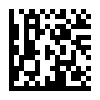
\includegraphics{img/dm_sample}
    \caption{Штрихкод в формате Data Matrix}
    \label{fig:dmSample}
\end{figure}

Каждый код Data Matrix содержит две сплошные пересекающиеся линии в 
виде буквы L, для ориентации считывающего устройства, две другие 
границы кода состоят из перемежающихся чёрных и белых точек и служат для 
указания размеров кода считывающему устройству 
(см. \figurename\ \ref{fig:dmPattern}). Размер кода может быть от
$10 \times 10$ до $144 \times 144$ барселей (существую также 
прямоугольные версии для цилиндрических поверхностей). Дополнительно
можно объединять до 16 кодов в один большой символ.
На рисунке \ref{fig:dmCoding} показано,
как размещаются байты в штрихкоде.

\begin{figure}[htb]
    \centering
    
\includegraphics{img/dm_pattern}
    \caption{Шаблон поиска в штрихкоде Data Matrix}
    \label{fig:dmPattern}
\end{figure}

\begin{figure}[htb]
    \centering
    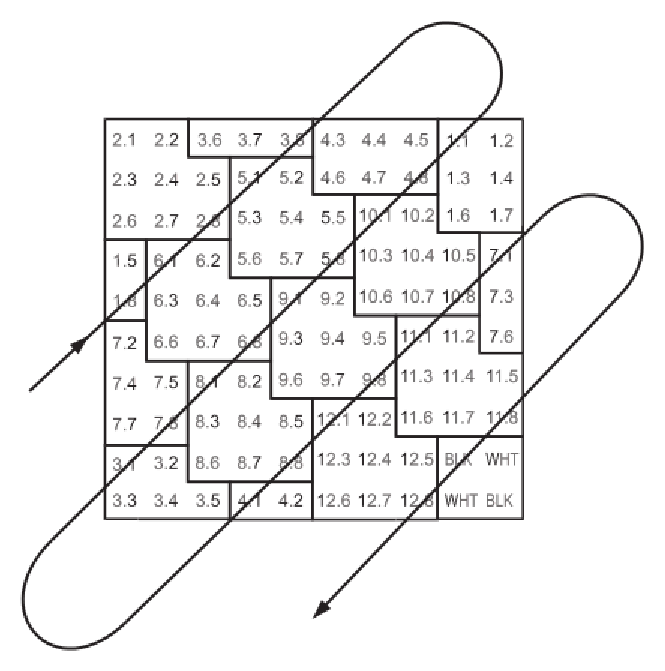
\includegraphics[scale=0.8]{img/dm_coding}
    \caption{Расположение байтов в Data Matrix}
    \label{fig:dmCoding}
\end{figure}

Все коды используют коррекцию ошибок стандарта ECC200, 
который, в свою очередь, использует алгоритм Рида-Соломона для 
кодирования/декодирования данных. Это позволяет восстановить в случае 
повреждения кода до 30\% полезной информации.

В промышленности Data Matrix применяют для маркировки различных элементов. 
Код может быть нанесён различными способами --- струйной печатью, гравировкой, 
лазером, электролитическими способами и т.д. В зависимости от метода нанесения, 
код может оставаться на элементе на протяжении всего его цикла 
использования (\figurename\ \ref{fig:dmSample2}).

\begin{figure}[htb]
    \centering
    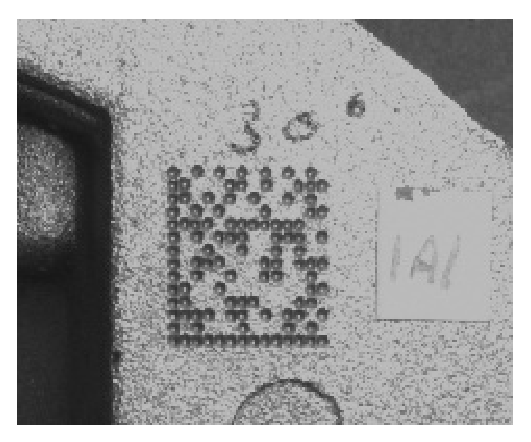
\includegraphics[scale=0.7]{img/dm_sample2}
    \caption{Штрихкод Data Matrix нанесённый методом иглографии}
    \label{fig:dmSample2}
\end{figure}

Основным положительным отличием Data Matrix от остальных двухмерных штрихкодов 
является то, что Data Matrix работает максимально быстро и небольшие объёмы 
данных осуществляются на минимальных площадях. Так, если кодировать 6 цифр, 
Data Matrix составит штрих-код размером $10 \times 10$ модулей, 
а вот если кодировать 
в Aztec, то эта площадь будет составлять $15 \times 15$ модулей. 
Но в то же время, 
данное преимущество теряется в процессе кодирования большего объёма информации: 
при одинаковых размерах символа в $132 \times 132$ модуля, Aztec закодирует  
почти 3000 
цифр, а Data Matrix максимум 2608. И при кодировании буквенно-цифровых данных 
в 10 символов, штрих-код Data Matrix занимает одинаковую площадь с Aztec. Чем 
же объясняется столь успешное кодирование малых пользовательских данных? Прежде 
всего, малым количеством служебной информации в составляемом коде, экономия 
производится за счёт размеров и структуры данных штрих-кода, таким образом 
надёжность считывания несколько падает. Также, Data Matrix имеет ещё один 
недостаток --- рост размера шаблона поиска символов увеличивается прямо 
пропорционально самому периметру символа, таким образом, становится невыгодным 
кодирование больших объёмов данных, у Aztec же шаблон поиска не изменяется.

\begin{table}[htb]
\centering
\caption{Таблица возможностей Data Matrix}
\begin{tabular}{|c|c|c|c|}
    \hline 
    Размер & \multicolumn{3}{c|}{Количество кодируемой информации} \\ 
    
    \hline 
    Ширина $\times$ Высота & Шифры & Символы & Байты \\
    
    \hline 
    $10 \times 10$ & 6 & 3 & 1 \\
    
    \hline 
    $12 \times 12$ & 10 & 6 & 3 \\
    
    \hline 
    $14 \times 14$ & 16 & 10 & 6 \\
    
    \hline 
    $16 \times 16$ & 24 & 16 & 10 \\
    
    \hline 
    $18 \times 18$ & 36 & 25 & 16 \\
    
    \hline 
    $20 \times 20$ & 44 & 31 & 20 \\
    
    \hline 
    $22 \times 22$ & 60 & 43 & 28 \\
    
    \hline 
    $24 \times 24$ & 72 & 52 & 34 \\
    
    \hline 
    $26 \times 26$ & 88 & 64 & 42 \\
    
    \hline 
    $32 \times 32$ & 124 & 91 & 60 \\
    
    \hline 
    $40 \times 40$ & 228 & 169 & 112 \\
    
    \hline 
    $44 \times 44$ & 288 & 214 & 142 \\
    
    \hline 
    $48 \times 48$ & 348 & 259 & 172 \\
    
    \hline 
    $52 \times 52$ & 408 & 304 & 202 \\
    
    \hline 
    $64 \times 64$ & 560 & 418 & 278 \\
    
    \hline 
    $72 \times 72$ & 736 & 550 & 366 \\
    
    \hline 
    $80 \times 80$ & 912 & 682 & 454 \\
    
    \hline 
    $88 \times 88$ & 1152 & 862 & 574 \\
    
    \hline 
    $96 \times 96$ & 1392 & 1042 & 694 \\
    
    \hline 
    $104 \times 104$ & 1632 & 1222 & 814 \\
    
    \hline 
    $120 \times 120$ & 2100 & 1573 & 1048 \\
    
    \hline 
    $132 \times 132$ & 2608 & 1954 & 1302 \\
    
    \hline 
    $144 \times 144$ & 3116 & 2335 & 1556 \\    
     
    \hline 
    \hline
    $8 \times 18$ & 10 & 6 & 3 \\
    
    \hline
    $8 \times 32$ & 20 & 13 & 8 \\
    
    \hline
    $12 \times 26$ & 32 & 22 & 14 \\
    
    \hline
    $12 \times 36$ & 44 & 31 & 20 \\
    
    \hline
    $16 \times 36$ & 64 & 46 & 30 \\
    
    \hline
    $16 \times 48$ & 98 & 72 & 47 \\
    
    \hline
\end{tabular} 
\end{table}
 

\subsubsection{Aztec Code}

Aztec Code представляет собой универсальную символику двухмерного
штрихового кода. Как показано на рисунках \ref{fig:acSmall} и \ref{fig:acBig},
код представляет собой квадрат, 
содержащий матрицу квадратных элементов, в центре которой располагается 
<<мишень>> (<<bullseye\footnote{Т.е. <<бычий глаз>> }>>), 
составленная из концентрических квадратов. Aztec 
позволяет эффективно кодировать как малые, так и большие объемы данных 
(цифры --- до 3832, текст --- до 3067 или байты --- до 1914) с 
использованием высокоэффективного метода Рида-Соломона коррекции ошибок 
(см. \ref{sec:RSCode}). Код Aztec разработан специалистами фирмы 
HandHeld Products (Andy Longacre и Rob Hussey) и защищен патентом, но частично 
выпущен для общего использования. Международная Спецификация Символики для 
кода Aztec утверждена AIM USA в формате ISO и доступна через филиалы AIM.



\begin{figure}[htb]
    \begin{multicols}{2}
 
        \begin{center}
             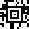
\includegraphics[]{img/ac_small} 
             \caption{<<Компактный>> символ Axtec Code}
             \label{fig:acSmall}
        \end{center}
   
        \begin{center}
            
\includegraphics[]{img/ac_big} 
            \caption{<<Полноразмерный>> символ Axtec Code}
            \label{fig:acBig}
        \end{center}       
       
    \end{multicols}
\end{figure}

Квадратная <<мишень>>, окружённая <<слоями данных>>, сплетенными с решеткой 
<<элементов привязк>>, расположенной по периметру квадрата, дают в результате 
изображения ассоциирующееся с искусством Центральной Америки, что и подсказало 
имя <<Aztec Code>> для символики. 

Основные изменения в структуре кода и коррекции ошибок появились в Версии 2.0 
спецификации в июне 1995 года, но основная конструкция кода осталась 
неизменной, выдержав процесс отладки считывающих устройств, пробные внедрения 
и даже критический анализ, проведённый Техническим Комитетом (Technical 
Symbology Committee) AIM USA без изменений. Международная спецификация 
Aztec Code опубликована AIM International в 1997 году.

Существуют два основных формата символа Aztec Code: <<Compact>> (Компактный) 
символ с мишенью из двух квадратов (\figurename\ \ref{fig:acSmall}) и 
<<Full-Range>> (Полный) символ с мишенью из трёх квадратов 
(\figurename\ \ref{fig:acBig}). Поскольку принтеры могут автоматически 
выбирать, а сканеры автоматически распознавать оба формата, вместе два формата 
образуют последовательность из символов 33 различных размеров, которые могут 
эффективно кодировать как малые, так и большие сообщения. В общем, 
символы Aztec Code:

\begin{enumerate}
\item могут кодировать любую байтовую последовательность в эффективных 
компактных режимах для текстовых и цифровых данных;

\item всегда квадратной формы, изменяясь в размерах от $15 \times 15$ 
модулей до $151 \times 151$ модулей. Свободной зоны вокруг символа не 
требуется вообще. Таблица \ref{tableAc} показывает информационную ёмкость 
некоторых размеров кода;

\item может быть использован в структурном объединении, соединяющем 
до 26 символов;

\item имеет специальный формат настройки сканера, удобный для 
настройки сканера с помощью штрихкода. 
 
\end{enumerate}

\begin{table}[htb]
%TODO Make it as text
\centering
\caption{Соотношения размеров символов и ёмкости Aztec Code}
\label{tableAc}
\end{table}

Вид символа Aztec Code очень систематичен с чётко разграниченными 
функциями частей, обеспечивает простоту процедур кодирования и 
декодирования, в то же время его математическая структура необычайно 
гибка и надёжна.

Рисунок \ref{fig:acStruct} показывает структуру полного символа 
Aztec Code. Вы можете увидеть три постоянных элемента:

\begin{enumerate}
\item центральный указатель <<мишень>>;

\item элементы ориентации по углам указателя;

\item решётка привязки, пронизывающая область данных.

\end{enumerate} 

\begin{figure}[htb]
    \centering
    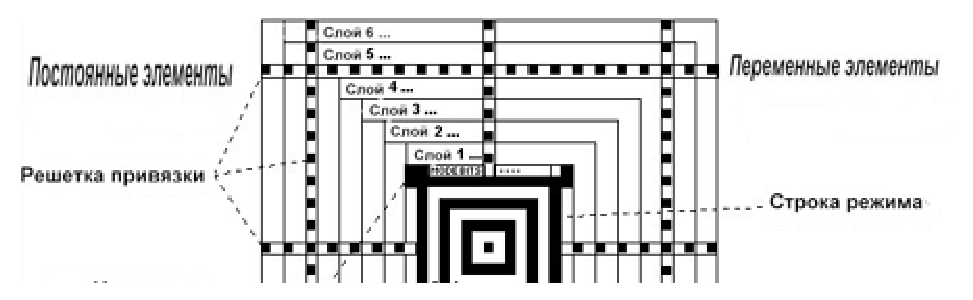
\includegraphics[scale=0.8]{img/ac_struct}
    \caption{Структура Aztec Code}
    \label{fig:acStruct}
\end{figure}
 
Два переменных элемента структуры\footnote{
Компактный символ Aztec Code содержит маленькую мишень без 
решётки привязки и только 4 слоя данных.} 
\begin{enumerate}
\item строка короткого режима, обернутая вокруг <<мишени>>;

\item от одного до 32 слоев данных толщиной в 2 барселя, 
спиралью расходящихся от центра.
\end{enumerate}

Строка короткого режима и слои данных закодированы с защитой от ошибок по 
методу Рида-Соломона. Строка режима --- это строка фиксированной длины, 
которая просто кодирует два параметра, несущие информацию о слоях данных, 
а именно: сколько слоев данных содержит данный символ и сколько слов 
содержится в сообщении (остаток места в области данных заполняется 
контрольными словами). Таким образом, уровень коррекции ошибок в Aztec Code 
становится регулируемым по указанию пользователя, и в принципе, слои 
данных могут содержать от 5\% до 95 \% контрольных слов, но на практике 
обычно нецелесообразно изменять стандартное значение в 23\% контрольных слов.

Слои данных, конечно, содержат последовательность кодовых слов, которые 
сперва кодируют пользовательские данные, затем добавляют к ним выявление и 
коррекцию ошибок. Защита от ошибок, кроме того, регулируемая пользователем 
и использующая дополнительные контрольные слова для заполнения, дополнительно 
усилена двумя путями: во-первых, размер кодового слова зависит от размера 
символа, от 6 бит для наименьших символов до 12 бит для наибольших, исключая 
необходимость чередующихся полей и обеспечивая хорошую зернистость для всех 
размеров символов. Во-вторых, слова сообщения, занимающие внешние слои символа, 
поддерживают чистовую коррекцию ошибок в стёртых углах символа.

В результате представленного рассмотрения технологии становятся понятными 
некоторые особенности Aztec Code: 

\begin{enumerate}
\item Слоёная природа полей данных обеспечивает целостность символов 33 
различных размеров и информационной ёмкости.

\item Указатель в виде мишени обеспечивает считывание при большом изменении 
угла сканирования.

\item Элементы ориентации дают возможность считывания при любой ориентации 
символа, включая зеркальное отражение. 

\item Решётка привязки позволяет учитывать существенные искривления 
больших символов.

\item Декодирование от центра к краю исключает необходимость полей 
(свободной зоны) вокруг символа.

\item Надёжный управляемый пользователем механизм коррекции ошибок по 
методу Рида-Соломона обеспечивает высокую производительность и надёжную 
защиту от ошибок. 

\item Расположение полей, устойчивых к появлению ошибок и повреждений, 
по краям символа, компенсирует влияние оптических искажений, возникающих 
по краям зоны сканирования.

\end{enumerate}

Aztec Code представляет собой универсальную символику 
матричного штрихового кода, хорошо приспособленную для визуальной технологии 
считывания и для кодирования как малых, так и больших объёмов данных. 
Aztec Code интересен для применений, требующих размещения кода на ограниченном 
пространстве (производство, коммерция, медицина, фармацевтика и т.д.), 
поскольку код обеспечивает высокую плотность размещения информации и не 
требует свободного пространства вокруг кода. Некоторые почтовые ведомства 
рассматривают возможность использования Aztec Code в качестве <<электронного 
штампа>> почтового отправления, в то же время электронное кодирование подписи 
с помощью Aztec привлекло внимание некоторых транспортных компаний.

\subsection{\textsc{Эффективность кода}}

\textit{Эффективностью штрихкода} $C$ назовём величину 

\begin{equation}
	\label{eq:theta}
	\theta_C(b, q) = \frac{b}{d(b, q)},
\end{equation}
где $d(b, q)$ ---
число барселей, которые необходимы для того, чтобы зашифровать сообщение
длинной $b$ бит при конфигурации кода $q$ (отражает 
уровень коррекции ошибок и т.д.). 

Другими словами, эффективность кода отражает число бит полезной
информации которое несёт в себе каждый барсель рассматриваемого 
кода $C$.

\textit{Предельной эффективностью кода} назовём величину

\begin{equation}
	\label{eq:Theta}
	\Theta_C(q) = \lim_{b \to \infty }\theta_C(b, q).
\end{equation}

Для рассмотренных выше кодов имеет место (принимаем во внимание,
что коды чёрно-белые, а значит один барсель~--- один бит):

\begin{equation*}
    d(b, q) = b + 2 \lceil b g(q) \rceil + f(b, q) + s (b, q),
\end{equation*}
где $g(q)$ --- текущий уровень коррекции ошибок (везде используется 
коды Рида-Соломона, поэтому на исправление одной ошибки требуется два 
дополнительных символа (см. \ref{sec:RSCode})), $f(b, q)$ --- свободное
место в матрице,  $s (b, q)$ --- служебная информация в коде\footnote{
В случае, когда каждый барсель может находиться в более чем двух состояниях
$k$ будем иметь:
\begin{equation*}
    d(b, q) = \frac{b+ 2 \lceil b g(q) \rceil}{\log_2 k}  + f(b, q) + s (b, q),
\end{equation*}
}. 
Принимая
во внимание тот факт, что $f(b, q) = o(b)$, a также $f(b, q) = o(b)$
(действительно, в рассматриваемых кодах информация записывается таким 
образом, что свободное место минимизируется; а служебные данные с возрастанием 
информации практически не возрастают) имеем\footnote{
Соответственно, для случая, описанного в предыдущем примечании:
\begin{equation}
	\Theta_C(q) = 
	    \frac{\log_2 k}{1 + 2g(q)}.
\end{equation}
}

\begin{equation}
	\Theta_C(q) = \lim_{b \to \infty } \frac
	    {b}
	    {b +2 \lceil b g(q) \rceil + o(b)} = 
	    \frac{1}{1 + 2g(q)}.
\end{equation}
\section{ОБЩИЕ ПРИНЦИПЫ ПОСТРОЕНИЯ И \\
РАСПОЗНАВАНИЯ ДВУМЕРНЫХ ШТРИХКОДОВ}

\subsection{\textsc{Коды Рида-Соломона}}
\label{sec:RSCode}

\subsection{\textsc{Перспективные преобразования}}

\subsection{\textsc{Общий алгоритм распознавания
двумерных штрихкодов}}
\section{ПОЛУТОНОВЫЕ МАТРИЧНЫЕ ШТРИХКОДЫ: \\
СПЕЦИФИКАЦИЯ, РЕАЛИЗАЦИЯ}

\subsection{\textsc{Спецификация полутонового матричного 
штрихкода}}

\subsection{\textsc{Пример реализации}}
%conclusion
\section*{ЗАКЛЮЧЕНИЕ}
\addcontentsline{toc}{section}{ЗАКЛЮЧЕНИЕ}

\newpage

%conclusion
\addcontentsline{toc}{section}{СПИСОК ИСПОЛЬЗОВАННЫХ ИСТОЧНИКОВ}
\renewcommand{\refname}{СПИСОК ИСПОЛЬЗОВАННЫХ ИСТОЧНИКОВ}

\begin{thebibliography}{99}
    \bibitem{bib:russkijLopatin} 
    \textit{Лопатин В.~В. и др.}  Русский орфографический словарь: 
    около 180 000 слов / Иванова О.~Е., Лопатин В.~В., Нечаева И.~В., 
    Чельцова Л.~К. Отв. ред. В. В. Лопатин. --- 2-е изд., испр. и доп. --- 
    М.: Институт русского языка имени В.~В. Виноградова РАН, 
    2004. --- 960 с.
    
    \bibitem{bib:isoQR}
    ISO/IEC 18004:2006. Information technology -- Automatic identification 
    and data capture techniques -- QR Code 2005 bar code symbology 
    specification.~--- 2 edition (Monolingual). --- 114 p. 
    
    \bibitem{bib:gostDM}
    ГОСТ Р ИСО/МЭК 16022 --- 2008. Автоматическая идентификация. Кодирование
    штриховое. Спецификация символики Data Matrix. ISO/IEC 16022:2006.
    Information technology -- Automatic identification and data capture
    tehniques -- Data Matrix bar code symbology specification (IDN).~--- 
    М., 2009 --- 125 с.
\end{thebibliography}

\begin{appendices}
    \section{ДИАГРАММА КЛАССОВ}

\section{ИСХОДНЫЙ КОД}


\end{appendices}
\end{document}